\begin{figure}[h]
    \centering
    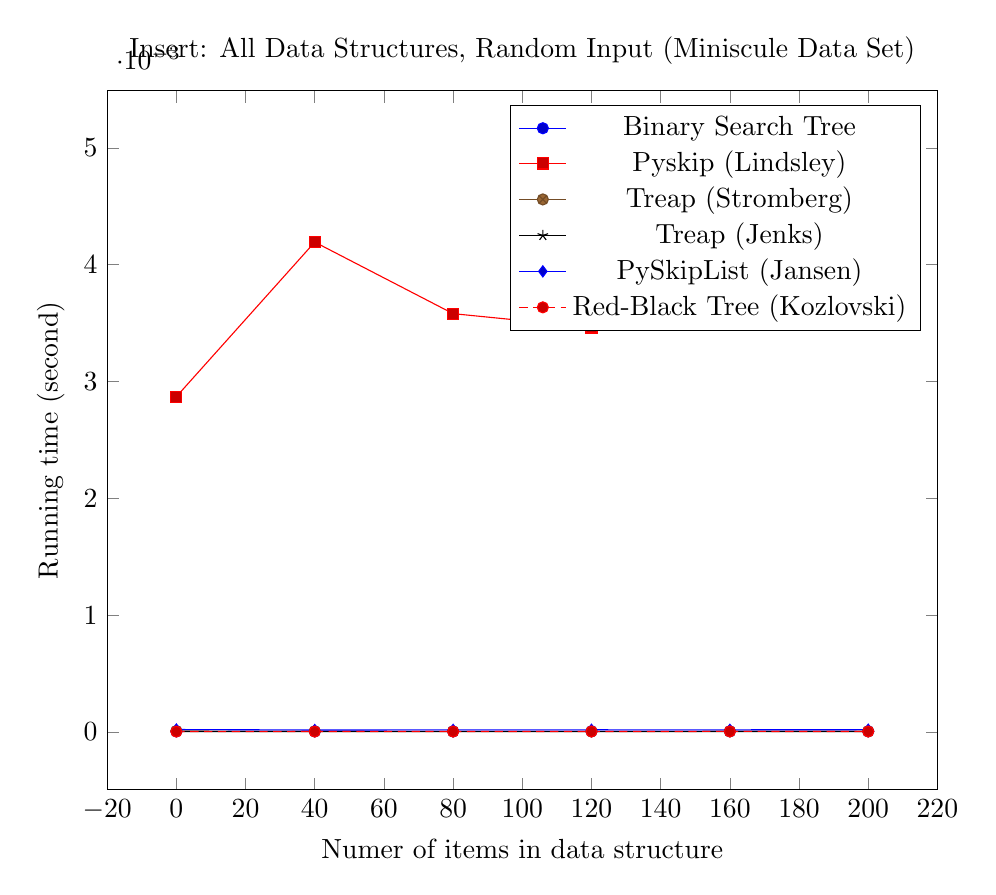
\begin{tikzpicture}
        \begin{axis}[
            xlabel={Numer of items in data structure},
            ylabel={Running time (second)},
            title={Insert: All Data Structures, Random Input (Miniscule Data Set)},
            width=\textwidth
        ]
		\addplot coordinates {
			(0, 4.306807315557215e-06)
			(40, 4.336924849224211e-06)
			(80, 4.0959845798216324e-06)
			(120, 4.9091579890525596e-06)
			(160, 4.728452787006176e-06)
			(200, 4.728452787006176e-06)
		};
		\addplot coordinates {
			(0, 0.002870261194310797)
			(40, 0.004193685859065011)
			(80, 0.00358103498904474)
			(120, 0.0034629742570380984)
			(160, 0.004989150158493505)
			(200, 0.004245518134519966)
		};
		\addplot coordinates {
			(0, 7.770323688172098e-06)
			(40, 5.330803460523726e-06)
			(80, 4.547747584959794e-06)
			(120, 4.397159916580406e-06)
			(160, 5.2103333258113335e-06)
			(200, 5.2404508594783294e-06)
		};
		\addplot coordinates {
			(0, 2.7406955644071474e-06)
			(40, 2.439520227692782e-06)
			(80, 2.2286974919349946e-06)
			(120, 2.3190500929803904e-06)
			(160, 2.108227357267012e-06)
			(200, 2.6202254297391647e-06)
		};
		\addplot coordinates {
			(0, 2.0299217697106188e-05)
			(40, 1.6293585718241132e-05)
			(80, 1.7016406526471074e-05)
			(120, 1.7919932536747396e-05)
			(160, 1.770910980098961e-05)
			(200, 1.8913811148024705e-05)
		};
		\addplot coordinates {
			(0, 2.7105780307845605e-06)
			(40, 2.9515183001649346e-06)
			(80, 3.102105968544322e-06)
			(120, 3.433398838970092e-06)
			(160, 3.945396911442245e-06)
			(200, 3.4936339063040834e-06)
		};
        \legend{Binary Search Tree, Pyskip (Lindsley), Treap (Stromberg), Treap (Jenks), PySkipList (Jansen), Red-Black Tree (Kozlovski)}
        \end{axis}
    \end{tikzpicture}
    \caption{Average of 10 operations, benchmarked every 40, starting at 0.}
\end{figure}